\documentclass[10pt]{article}

%\usepackage[a4paper,left=2cm,right=2cm,top=1.5cm,bottom=2cm]{geometry}
\usepackage{graphicx}
\usepackage{listings}
\usepackage{amsmath}
\usepackage{algorithm}
\usepackage{algpseudocode}
\usepackage[backend=biber]{biblatex}
\addbibresource{references.bib}
\setlength{\oddsidemargin}{1.8cm}

\begin{document}

${ \ } $ \vspace{4cm}
%
%% Titlepage 1 
%

\begin{center}
{\huge \bf Playing video games using neural networks and reinforcement learning}
\end{center}

\begin{center}
{\large \bf Joseph Shihab Esmaail}
\end{center}

\begin{center}
May 2016
\end{center}

\vspace{2.5cm}

\begin{abstract}
This is a Technical Computer Science project, with the aim to develop a neural network that is able to learn to play video games. This document explains the projects motivations and aims, what related work exists, my current understanding of the theory and tools involved, and how the development of the project will be handled. (edit and not exceed 10 lines)
\end{abstract}


\vfill

\begin{center}
Project Dissertation submitted to Swansea University\\
in Partial Fulfilment for the Degree of Bachelor of Science
\end{center}

\begin{center}

\includegraphics[scale=0.2]{img/logo.png}
\end{center}

\begin{center}
Department of Computer Science\\
Swansea University
\end{center}

\thispagestyle{empty}

\newpage

\thispagestyle{empty}

\section*{Declaration}

This work has not previously been accepted in substance for any degree
and is not being currently submitted for any degree.

\vspace{0.5cm}
\begin{tabular}{l}
\today\\
\\
Signed:
\end{tabular}

\section*{Statement 1}
This dissertation is being submitted in partial fulfilment of the
requirements for the degree of a BSc in Computer Science.

\vspace{0.5cm}
\begin{tabular}{l}
\today\\
\\
Signed:
\end{tabular}

\section*{Statement 2}

This dissertation is the result of my own independent
work/investigation, except where otherwise stated. Other sources are
specifically acknowledged by clear cross referencing to author, work,
and pages using the bibliography/references. I understand that failure
to do this amounts to plagiarism and will be considered grounds for
failure of this dissertation and the degree examination as a whole.

\vspace{0.5cm}
\begin{tabular}{l}
\today\\
\\
Signed:
\end{tabular}

\section*{Statement 3}

I hereby give consent for my dissertation to be available for
photocopying and for inter-library loan, and for the title and summary
to be made available to outside organisations.

\vspace{0.5cm}
\begin{tabular}{l}
\today\\
\\
Signed:
\end{tabular}

\newpage
\tableofcontents
\newpage

\section{Introduction}
	Neural Networks are a model within the field of Machine learning which is currently a major buzzword in the Computer Science Discipline, owing a lot to the recent growth of big data. It has also gained increasing public presence through efforts such as IBM's Watson, which won against two former champions in Jeopardy in 2011, and Google's DeepDream program which displayed how convolutional neural networks interpret images.\\
	Machine learning is also a major player in our day to day lives with Apple, Microsoft, and Google all using it for their smartphone digital assistants, Google using it for their search engine, and social media such as Facebook using it to cater it's service to each individual user. This will also extend in the coming future with autonomous vehicles such as Google's self-driving car project and motor companies such as Tesla starting to incorporate self-driving systems into their cars.\\
	
	This project aims to apply machine learning, in particular neural networks, to the task of learning to play video games. Video games have been an almost constantly growing phenomenon since their inception in the 1970's with Pong, recently entering the mainstream with the growth of the eSports industry which hosts tournaments with prize pools in the region of a million US dollars. The application of machine learning to video games has the potential to enable a greater interest in machine learning, as it's current implementations is very pervasive.\\
	
	 This dissertation will provide the reader with a background to neural networks, reinforcement learning and relating work to these and their application to video games, as well as how this project has been organised, what technologies are utilised, how the task has been approached and implemented, as well as what results are produced.
	
	%In one or two paragraphs, introduce the topic. Followed immediately with why it is a useful project, possible applications of the work. Question == "What is this dissertation topic good for?"\\
	
	%Present the benefits, advantages and novelty of the diss.\\
	%Who will potentially benefit from the work?\\
	%what does the reader gain from reading the diss?\\
	
	%Inherited advantages from previous systems/algorithms may be listed\\
	
	%specific challenges to overcome (conceptual and technical) mentioned\\
	
	%concludes with how the rest of the dissertation is organised.	
\medskip

\subsection{Aims and objectives}
	%restate the aims and objectives from the intial and interim docs
	To be able to successfully produce a neural network that can play video games, the network will need a way to interact with the video games, both to receive information about the current game state and to send actions into the video game to play. So we will need methods to obtain the outputted game screen data and current score, as well as methods to input actions as a human player would via a game controller. The neural network needs to be able to interpret the input game state, and output a decision on what action to perform, this action hopefully being one that results in the best performance or score in the video game. The neural network will determine what action is the optimal one after performing a learning process using reinforcement learning, on the particular video game in question. After the network is capable of performing optimal actions to the best of its ability, the performance will be evaluated against human players to make a decision on how successful it was at learning to play the video game.\\
	
	To summarise, the aim of this project is to develop an artificial intelligence agent, namely a neural network that will use reinforcement learning to learn to play a large set of video games. This can be achieved by splitting the overall task into the following steps:
	
	\begin{itemize}
		\item Find methods to manipulate video game inputs and outputs.
		\item Develop the neural network.
		\item Develop reinforcement learning methods for the intelligence agent.
		\item Train and evaluate the neural network with video games.
		\item GPU-Accelerate the network to improve performance.
	\end{itemize}
	
	\bigskip

\section{Literature review}
	%research done in order to prepare for the project
	
	%\subsection{Related work}
		%choose proper scope, choose which books/papers to refer to and which to ignore. Each previous publication gets a one paragraph description.
		
		An early use of a neural network to play a game can be seen in the paper `Temporal difference learning and TD-Gammon' by Gerald Tesauro. In this Tesauro applies the neural network (known as TD-Gammon) to the game backgammon, and trained itself using reinforcement learning, in particular \textit{temporal-difference learning}. The neural network would train itself ``by playing against itself and learning from the outcome" \cite{tdgammon}. Tesauro concludes that the temporal difference learning proved to be ``a promising general-purpose technique" \cite{tdgammon}. TD-Gammon successfully learnt to play backgammon, successfully enough that ``by version 2.1 TD-Gammon was regarded as playing at a level extremely close to equalling that of the best human player, and had even started to influence the way expert backgammon players played" \cite{tdgammon}. This particular implementation of reinforcement learning to neural networks however would not be possible to implement across a broad selection of games as it requires a game with two players.\\
		
		Neural networks and reinforcement learning have also been applied to obstacle avoidance in robots, which is a similar environment to that of video games. In the paper `Reinforcement learning neural network to the problem of autonomous mobile robot obstacle avoidance' by Huang et al.  reinforcement learning was chosen because ``a complete knowledge of the environment is not necessary" \cite{rlrobot}. When a human player starts to learn to play a video game, they also do a complete knowledge of all the elements of the game. In this case the neural network needs to be learning the video game in a similar fashion to how a human player would, so reinforcement learning is applicable here. The results of the paper show that using neural networks and reinforcement learning can enhance learnability and allow task completion in a complex environment, which can also be translated across to the application to video games.\\

		In 2007 the paper `Reinforcement learning and neural networks for Tetris' by Nicholas Lundgaard and Brian McKee saw the application of neural networks and reinforcement learning to the popular 1984 video game Tetris. They observe that video games are well suited for the application of reinforcement learning as more often than not there is a built in system to track how well a player is doing, often known as the score or points of the player. They also make the observation that in the case of Tetris ``it is nearly impossible to definitively say what was a right or wrong move" \cite{rlnntetris}, which can be applied also to most video games and means that the task of learning for neural networks applied to them cannot be done through supervised learning. In practice they found that ``while the learning agents fail to accumulate as many points as the most advanced AI agents, they do learn to play more efficiently"\cite{rlnntetris}. Lundgaard and McKee conclude that ``compared to human performance, the learning agents appear to perform well: while they can't survive forever, they perform better during game-play"\cite{rlnntetris}. This suggests that an AI player doesn't necessarily gain an unfair advantage over a human player by being capable of surviving indefinitely, they instead play at a similar pace.\\
		
		The most recent and relevant work in developing neural networks to play video games comes from DeepMind, who were recently acquired by Google. Initially in their paper `Playing Atari with deep reinforcement learning' in 2013 and then expanded upon in 2015 in `Human-level control through deep reinforcement learning', a paper which made the front page of Nature. In these papers they refer to their neural network as a Deep Q network (DQN), which is a deep convolutional neural network trained using a variant of Q-learning. This network is then applied to Atari 2600 games via the \textit{Arcade learning environment}, which was also developed by DeepMind. A convolutional neural network was chosen here because it ``mimics the effects of receptive fields"\cite{humanlevel}, so it is more equipped for the task of pattern recognition within images. A deep network was chosen because ``several layers of nodes are used to build up progressively more abstract representations of the data"\cite{humanlevel}, allowing the network to ``learn concepts such as object categories directly from the raw sensory data"\cite{humanlevel}. The results of this paper show that their ``DQN method outperforms the best existing reinforcement methods on 43 of the games" \cite{humanlevel}. As well as this they report that their agent ``performed at a level that was comparable to that of a professional human games tester" \cite{humanlevel}.\\
		
		 A selection of the DQNs performances are shown in figure \ref{fig:performance}, the values for which are ``normalised with respect to a professional human games tester (that is, 100\% level) and random play (that is, 0\% level)." \cite{humanlevel}. Figure \textbf{create it} in the appendix displays the performance for all 43 games.
		
		\begin{figure}[h]				
			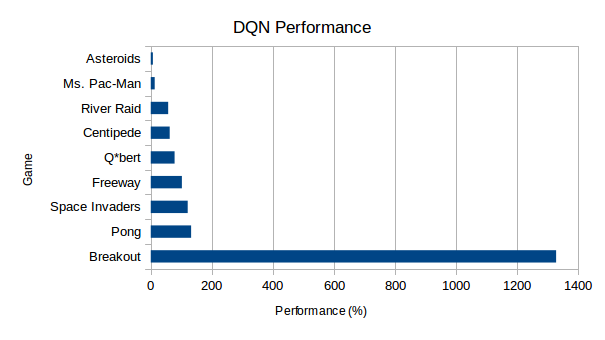
\includegraphics[scale=0.7]{img/deepMindPerformance}
			\centering
			\caption{DQN performance with regard to human performance \cite{humanlevel}.}
			\label{fig:performance}
		\end{figure}
		
		This related work confirmed that a neural network is a suitable model of machine learning to apply to the task of learning to play video games. In particular a deep convolutional neural network trained with a Q-learning variant has been proven as capable of learning to play multiple video games as opposed to just one, with no changes to the structure of the neural network.\\
		
	\bigskip
	
	\section{Neural networks}
	%From the ground up, how nns work. Talk about various different types of neural networks and training methods.
		Neural networks (also known as artificial neural networks) are machine learning models based on the structure of the brain in animals such as humans.\\
		
		\begin{figure}[h]			
			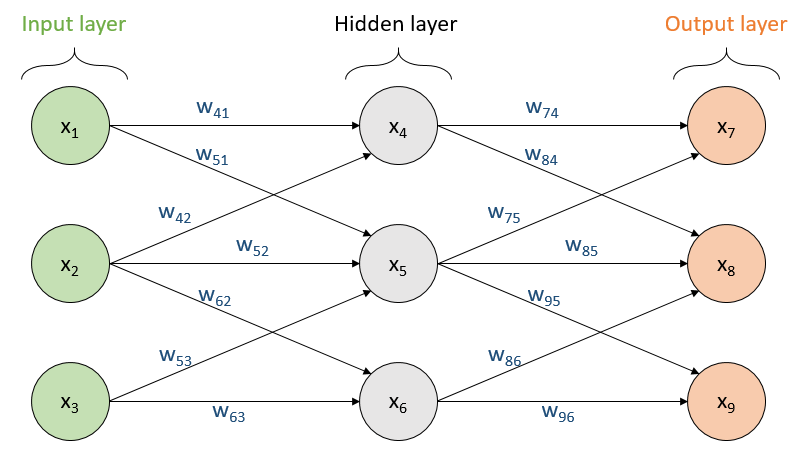
\includegraphics[scale=0.5]{img/network}
			\centering
			\caption{An example neural network.}
			\label{nnetwork}
		\end{figure}	
		
		These neural networks are, naively, a collections of connected nodes, where the nodes are referred to as neurons, and the connections between them as weights. The neurons of the network exist in layers, an input layer for inputs to the network, and output layer to give the results of the network, and potentially some hidden layers in between. If a neural network has more than one hidden layer that network is then considered a Deep neural network. A neural network is a feed-forward network if all of it's connections point towards the output layer, or a recurrent network if there exist feedback connections which point backwards in the network towards the input layer. For the purpose of this explanation I will be using a feed-forward network,\\
		
		The input layer of the neural network receives its data from the input to the network, this data is then passed along weighted connection(s) to neurons in the next layer of the network. All layers of a network, with the exception of the input layer, have a bias unit as well as having a summation and an activation function performed on them before the neuron data is propagated forward through to the next layer. The summation process for a neural is performed as follows:
		\begin{equation}
			x_i = \sum_{j} w_{ij} x_j + b 
		\end{equation}
		Where:
		\begin{list}{•}{•}
			\item $w_{ij}$ represents the weight for the connection from neuron $j$ to neuron $i$.
			\item $x_j$ is the value of neuron $j$.
			\item $b$ is the value of the bias unit.
		\end{list}
		
		After this summation process is applied to a neuron an activation function is usually applied. The most commonly applied activation function, and the one i will use for this explanation, is a Sigmoid function which is visualised in Figure \ref{sigmoid}. A Sigmoid activation would be performed as follows:\\
		\begin{equation}
			\sigma(z) \equiv \frac{1}{1+e^{-z}}
		\end{equation}
		
		\begin{figure}[h]			
			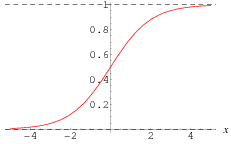
\includegraphics[scale=0.75]{img/sigmoid}
			\centering
			\caption{Graph of the Sigmoid function \cite{sigGraph}}
			\label{sigmoid}
		\end{figure}
		
		The summation and activation function for a neuron can be combined into one calculation for the final output value of a neuron as:\\
		\begin{equation}
			output(x_i) = \sigma (\sum_j w_{ij} x_{j} + b)
		\end{equation}	
		\begin{equation}
			\sigma(z) \equiv \frac{1}{1+e^{-\sum_j w_{ij} x_{j} + b}}
		\end{equation}
		
		Once the values have been propagated to the output layer and the neurons in the output layer have had summation and activation performed on them, we have the output of the neural network.\\
		
		\medskip
		
		\subsection{Convolutional neural network}
		
		 There are many different types of neural networks as well as just feed-forward and recurrent, for the purposes of this dissertation, I am using a convolutional neural network. Convolutional neural networks are design to ``recognise two-dimensional shapes with a high degree of invariance to translation, scaling, skewing, and other forms of distortion" \cite{nncomp}. These convolutional neural networks use the main concepts of shared weights and biases, local receptive field, and very often, max pooling. The input for this kind of network would be the pixels of an image, for example, a 25x25 greyscale image would have an input layer size of 25x25, a sequence of 3 25x25 greyscale images would have an input layer size of 25x25x3.\\
		 
		 Unlike a normal neural network, convolutional neural networks have layers known as convolutional layers, which are either a 2 or 3 dimensional structure. These convolutional layers use local receptive fields which connect ``the input pixels to a layer of hidden neurons. However we won't connect every input pixel to every hidden neuron. Instead we only make connections in small, localised regions of the input image"\cite{nndl}.\\
		 
		\begin{figure}[h]				
			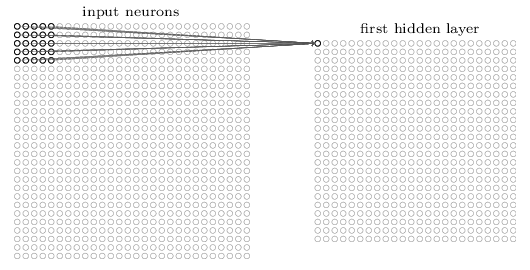
\includegraphics[scale=0.55]{img/convNet1}
			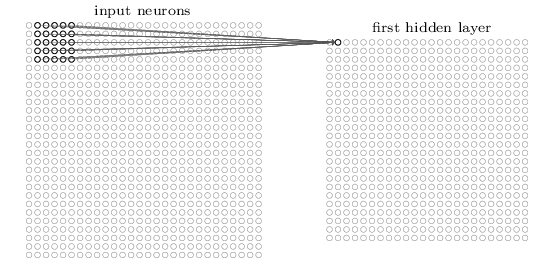
\includegraphics[scale=0.55]{img/convNet2}
			\centering
			\caption{How local receptive fields work \cite{nndl}}
			\label{fig:lrf}
		\end{figure}
		Figure \ref{fig:lrf} visualises how a local receptive field of size 5x5 with a stride length of 1 works. The stride length is the amount of pixels we shift the local receptive field when applying pixels to the next hidden layer neuron. The size of the local receptive field is also then the size of the shared weights for the convolutional layer. These shared weights are used for every local receptive field in the current layer as well as a shared bias. The process for summation and activation of the result of a convolutional layer can expressed as \cite{nndl}:
		\begin{equation}
			\sigma (b + \sum^4_{l=0} \sum^4_{m=0} w_{l, m} x_{j+l, k+m})
		\end{equation}
		Where a 5x5 local receptive field is being applied for the $j^{th}, k^{th}$ hidden neuron with $\sigma$ as the activation function, $w_{l, m}$ as the shared weights, and $x$ represents the value of the input neuron \cite{nndl}.\\
		
		Convolutional neural networks can also have pooling layers, which can be ``used immediately after convolutional layers" \cite{nndl}. While these layers do no actual learning, they can perform a process known as max pooling. A max pooling layer will take the output of the convolutional layer (size $N*N$), extract the maximum of a $k8k$ region, and output a $\frac{N}{k} * \frac{N}{k}$ layer \cite{convNN}.\\
		
		A Convolutional network can be made up of a sequence of convolutional layer followed by pooling layers and then normal feed-forward neural network layers such as fully connected layers, where every neuron in the current layer is connected to every neuron on the previous layer. You can also omit the pooling layer, particularly in the case of applying to low resolution images, and just use a sequence of convolutional layers followed by normal feed-forward layers.\\
		
		\medskip
		
		\subsection{Backpropagation}
		
		The details covered so far only cover the forward propagation of a neural network, the network needs to also propagate backwards and tune parameters such as weights and biases to present a more meaningful output to given input, also known as learning. There are, generally speaking, three kinds of learning that can be applied in machine learning, supervised learning, unsupervised learning, and reinforcement learning.\\
		 Supervised learning requires ``the availability of a teacher or supervisor who classifies the training examples into classes" \cite{nnintell}. For unsupervised learning the network ``must identify the pattern-class information as a part of the learning process" \cite{nnintell}. Reinforcement learning uses the idea of states, actions and rewards, and encourages the network to perform actions in states that produce the greatest reward.\\
		 
		 To actually be able to utilise any of these learning methods, the neural network needs to apply an algorithm to actually perform the learning process, the most popular of which is backpropagation. The output of the neural network is highly unlikely to be correct on the first run of the network, due to the weights and biases of the network being assigned randomly at the start. We require a method to bring the actual output of the network closer to the desired output. This is backpropagation and is done using gradient descent.\\
		 Once the neural network has been run on several pieces of input data, we want to see how different the actual output is from the desired output. This error is calculated as \cite{bpexample}:
		\begin{equation}\label{eq:total}
			E_{total} = \sum \frac{1}{2}(target-output)^2
		\end{equation}
		\begin{equation}\label{eq:indiv}
			E_{O_i} = \frac{1}{2}(target_{O_i} - output_{O_i})
		\end{equation}
		Equation \ref{eq:total} is for the total error of all output neurons, and equation \ref{eq:indiv} is for the error for one output neuron $i$.\\
				
		The idea behind backpropagation is to find how much to change the weights and biases so that the actual output can be brought closer to the desired output. The process for this differs depending on if it is applied to an output layer, or to a hidden layer of the network.\\
				
		When applying it to an output layer we want to find how much to change the weight $w_{ij}$, that connects a hidden neuron $j$ to an output neuron $i$, to correct our output. So we need to calculate the change in $E_{total}$ with regard to $w_{ij}$, this can be done with derivatives.
		\begin{equation}\label{eq:deriv}
			\frac{\partial E_{total}}{\partial w_{ij}}
		\end{equation}
		\begin{equation}\label{eq:chain}
			\frac{\partial E_{total}}{\partial w_{ij}} = \frac{\partial E_{total}}{\partial out_{O_i}} * \frac{\partial out_{O_i}}{\partial net_{O_i}} * \frac{\partial net_{O_i}}{\partial w_{ij}}
		\end{equation}
		Here we apply the chain rule to (\ref{eq:deriv}) to get (\ref{eq:chain}) \cite{bpexample}. $net_{O_i}$ is the net output of the output neuron $i$ before the activation function has been applied.\\
		
		Next we calculate the change in the $E_{total}$ with regard to $out_{O_i}$, the change in $out_{O_i}$ in regard to $net_{O_i}$, and the change in $net_{O_i}$ with regard to $w_{ij}$ \cite{bpexample}.
		\begin{equation}
			\frac{\partial E_{total}}{\partial out_{O_i}} = -(target_{O_i} - out_{O_i})
		\end{equation}
		\begin{equation}\label{eq:derAct}
			\frac{\partial out_{O_i}}{\partial net_{O_i}} = out_{O_i}(1 - out_{O_i})
		\end{equation}
		\begin{equation}
			\frac{\partial net_{O_i}}{\partial w_{ij}} = out_{H_j}
		\end{equation}\\
		\begin{equation}\label{eq:OutFinal}
			\frac{\partial E_{total}}{\partial w_{ij}} = -(target_{O_i} - out_{O_i}) * out_{O_i}(1 - out_{O_i}) * out_{H_j}
		\end{equation}
				 
		In (\ref{eq:derAct}), the derivative of the activation function(sigmoid) has been calculated which is "the output multiplied by 1 minus the output" \cite{bpexample}.\\
				 
		(\ref{eq:OutFinal}) can then also be written with the \textit{delta rule} \cite{bpexample}.			 
		\begin{equation}
			\delta_{O_i} = \frac{\partial E_{total}}{\partial out_{O_i}} * \frac{\partial out_{O_i}}{\partial net_{O_i}} = \frac{\partial E_{total}}{\partial net_{O_i}}
		\end{equation}
		\begin{equation}
			\frac{\partial E_{total}}{\partial w_{ij}} = \delta_{O_i}out_{H_j}
		\end{equation}\\
		
		\medskip
		
		When applying backpropagation with gradient descent to a hidden layer, the process can be sped up by making use of the delta rule. We want to find the change in $E_{total}$ with regard to $w_{ij}$, a weight connecting neuron $j$ (can be in either input or hidden layer, depending on position in network) to neuron $i$ in a hidden layer. \cite{bpexample}
				
		\begin{equation}
			\frac{\partial E_{total}}{\partial w_{ij}} = \delta_{H_i} * \frac{\partial net_{H_i}}{\partial w_{ij}}
		\end{equation}
		\begin{equation}
			\frac{\partial net_{H_i}}{\partial w_{ij}} = out_j
		\end{equation}
		\begin{equation}
			\frac{\partial E_{total}}{\partial w_{ij}} = \delta_{H_i} * out_j
		\end{equation}\\
				
		Now to get our new value of $w_{ij}$, $w^+_{ij}$ we perform the following \cite{bpexample}:
		\begin{equation}
			w^+_{ij} = w_{ij} - \eta * \frac{\partial E_{total}}{\partial w_{ij}}
		\end{equation}
		With $\eta$ being a learning rate for the neural network.\\
		
		\medskip

		The learning method that will be used for this dissertation is backpropagation but implemented using a method known as RMSProp \cite{rms}\ a variant of Stochastic gradient descent. Stochastic gradient descent differs from normal gradient descent by applying to a random subset of training data as opposed to all of it. This approach is advantageous when you have a very large training set and/or a large amount of weights to update. RMSProp then builds upon this, it will ``divide the learning rate for a weight by a running average of the magnitudes of recent gradients for that weight" \cite{rms}. This particular method has been chosen as it has been proven to work in the application of neural networks to video games in the paper `Human-level control through deep reinforcement learning' \cite{humanlevel}.\\
	
	\bigskip
	\section{Reinforcement learning}
	%Discuss the general idea of reinforcement learning, then Q-learning and then DQNs
		The learning method that will be utilised for the neural network in this project is Reinforcement learning. Reinforcement learning, as mentioned above, uses the idea of states, actions, and rewards to encourage the network to perform actions that produce the best possible reward for their current state. It is a learning model reminiscent of how animals learn, ``learning what to do - how to map situations to actions - so as to maximise a numerical reward signal" \cite{rlintro}. A machine learning model using reinforcement learning is able to enter an unknown situation and ``learn from it's own experience" \cite{rlintro}.\\
		
		\medskip
		
		\subsection{Q-learning}
		The particular method of reinforcement learning that is implemented here is Q-learning. In Q-learning we attempt to find the optimal action for each state to maximise the reward gained. This kind of learning very closely matches the basic idea of how to learn to play a video game. The way that Q-learning works is that ``for every possible state, every possible action is assigned a value which is a function of both the immediate reward for taking the action and the expected reward in the future based on the new sate that is the result of taking that action" \cite{qlearning}. The value update function for this, as found in \cite{qlearning}, is as follows:
		\begin{equation}\label{eq:qlearn}
			Q(x,u) := (1 - \alpha)Q(x,u) + \alpha(R + \gamma maxQ(x_{t+1},u_{t+1}))
		\end{equation}				
		Where, 
		\begin{list}{•}{•}
			\item $Q$ is the expected value of performing action $u$ in state $x$,
			\item $R$ is the reward,
			\item $\alpha$ is the learning rate,
			\item $\gamma$ is the discount factor.
		\end{list}
		This dissertation will use the neural network as a function approximator for Q-learning. This means that each input to the network (game screen data) will be treated as a state, and the output of the network (the action to perform in game) will be treated as an action, with an associated reward. The value update as seen in equation \ref{eq:qlearn} will then be applied. The neural network used is therefore referred to as a Deep Q network.
		
		\bigskip
	
\section{Project Management}
	\subsection{Software life-cycle*}
		The software life-cycle used for this project is the agile development model, in particular the scrum model. The choice of agile for this project is advantageous compared to a more traditional model such as waterfall. This is because in the Waterfall model ``as the requirements change or as requirements problems are discovered, the system design or implementation has to be reworked and retested" \cite{swengi}. This would be particularly problematic and result in a prolonged development process if and when errors occur, especially in earlier stages as it may in a undergraduate project such as this.\\
		
		\begin{figure}[h]			
			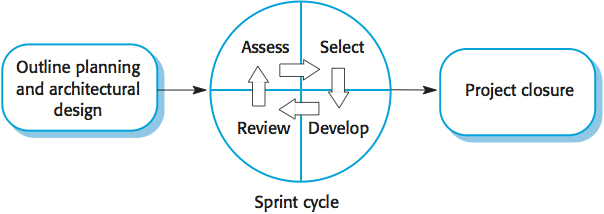
\includegraphics[scale=1]{img/scrum}
			\centering
			\caption{The Scrum development process \cite{swengi}}
			\label{scrum}
		\end{figure}
		
		The Scrum method is designed for small development teams, as a result many elements of scrum have been scaled down or omitted completely for application to this project. For example, there are several different roles for development team members such as a Scrum master, in this case the roles have been removed altogether.\\
		
		Development in the scrum method is performed as displayed in figure \ref{scrum}, beginning with the outline planning stage. Here we establish the project's general objectives and design the software architecture. In this case, this stage was undertaken during the initial document. Next follows the main area of scrum, the sprint cycle. It is within this sprint cycle that the actual development is performed, and is done so in a series of fixed-length sprints. These sprints are then divided into four phases:
		
		\begin{enumerate}
			\item \textbf{Assessment phase}: A list of tasks to be performed on the project is reviewed, priorities and risks are assigned to them. In the review of tasks, more may be added.
			\item \textbf{Selection phase}: The task or tasks to be performed this sprint cycle are chosen.
			\item \textbf{Development phase}: Progress is reviewed at regular intervals, and task priorities can be potentially re-assigned.
			\item \textbf{Review phase}: Tasks performed this cycle are now reviewed.\\
		\end{enumerate}
		
		The final stage of scrum is then project closure, this wraps up the project with required documentation being produced and lessons learnt from the project are assessed. The project closure process is this final dissertation document for the project.\\
		
		I feel that scrum has been beneficial to the development of this project as it broke it down into smaller digestible sprints. Each sprint had clear goals set out, prioritised and then reviewed. It has also meant that there is less chance for any delay in development as there have been regular stops to review and reassess the tasks being performed.
	
	\medskip
	
%	\subsection{Development*}
%	%Rename to development and discuss windows dev and linux run?
%	%BCCC
%	
%	\textbf{IS THIS SECTION NECESSARY?}
%	
%	This project is developed in the C++ language. The development will be performed within the Windows Operating System and the project will be compiled and run within Linux. Windows is being used for development because it allows for usage of the Visual studio 2013 integrated development environment. This is preferable as it offers a built-in compiler and debugger for C++ as well as Intellisense code completion. Linux is then used for the final compilation and running of the project as tool to access video games and their data, the Arcade learning environment, is not compatible with Windows.\\
%	
%	All code produced for this project will conform to `Bob's concide coding conventions' \cite{bc3} as outlined by Dr. Robert S Laramee of Swansea University.\\
%	
%	\medskip
	
	\subsection{Project timeline}
	%Discuss risks and how they have come in, and use the gantt chart!
	
		\begin{figure}[h]				
			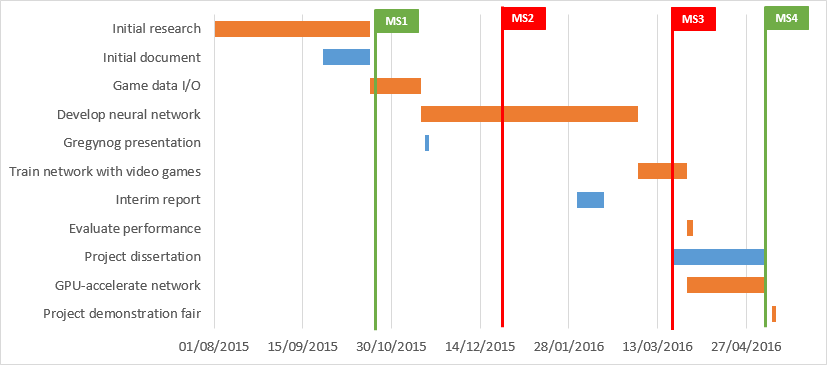
\includegraphics[scale=0.6]{img/newSchedule}
			\centering
			\caption{Planned project schedule.}
			\label{fig:newSchedule}
		\end{figure}
		
		\begin{center}
			\begin{tabular}{ c | p{3.5cm} | c }
				\textbf{Label} & \textbf{Milestone} & \textbf{Reason} \\ \hline
				MS1 & End of initial phase, start of sprint cycle. & Scrum development model.\\ \hline
				MS2 & Start of Christmas break. & Allows more time dedication to project.\\ \hline
				MS3 & Start of Easter break. & Allows more time dedication to project.\\ \hline
				MS4 & End of project closure phase. & Scrum development model.					 
			\end{tabular}
		\end{center}		
		The project schedule, as seen in figure \ref{fig:newSchedule}, has 2 kinds of tasks. Tasks set by the Computer Science department are those with blue bars, and tasks as set out by myself are those with orange bars. There are also 2 kinds of milestones, green milestones which represent the end of the intial and closure phases of scrum, and red milestones which represent the two holiday breaks in University term time. This breaks have allowed me to allocate more time to the development of the project and/or completion of documentation for the project. The bulk of the time for the project plan was dedicated to the development of the neural network in C++. This is both because it is the most integral component of this project, and because I required to learn the C++ language as I had no prior usage of it until this project.\\
		
		The way that the project development actually took place can be seen in figure \ref{fig:actSchedule}. Here the tasks of `Train network with video games', `Evaluate performance', and `GPU-accelerate network' have been removed as the actual implementation of the network did not finish so these tasks could not then be performed.\\
		
		\begin{figure}[h]				
			\includegraphics[scale=0.6]{img/finalSchedule}
			\centering
			\caption{Actual project schedule.}
			\label{fig:actSchedule}
		\end{figure}
		
	\medskip
		
	\subsection{Risks}
	%Risk tables and perhaps discussion on risks that actually happened, if they were expected or not before outlined!
	\begin{figure}[h]
		\begin{tabular}{ p{4.5cm} | c | c | c | p{4.5cm} }
			\multicolumn{1}{c}{\textbf{Risk}} & \textbf{P} & \textbf{I} & \textbf{Score} & \multicolumn{1}{c}{\textbf{Mitigation}}\\ \hline
			Project is too ambitious. & 8 & 8 & 64 & Scale back/adjust project aims.\\ \hline
						
			Illness of close family member that will require my care. & 5 & 6 & 30 & Have good time management to afford missed days and/or catching up.\\ \hline
			GitHub has a service failure. & 3 & 7 & 21 & Keep sufficient offline backups of project development\\ \hline			 
			Development slowed due to Migraines. & 6 & 3 & 18 & Have good time management to afford missed days and/or catching up.\\ \hline 
			General illness. & 5 & 3 & 15 & Have good time management to afford missed days and/or catching up.\\ \hline
			Hardware failure. & 2 & 5 & 10 & Keep sufficient backups of files, and spares for components.					 
		\end{tabular}		
		\caption{Risk table}
		\label{fig:newRisks}
	\end{figure}
	
	The risks involved in the development of this project can be seen in the risk table in figure \ref{fig:newRisks}, with `P' representing the Probability of the risk (scaled from 1 to 10), `I' representing the Impact of the risk (scaled from 1 to 10), and `Score' representing the Risk score, which is calculated as the product of the probability and impact of the risk, and the risks are ordered by this risk score.\\
	
	The risks of this project are mostly all relating to some kind of down time. In the case of myself getting ill, be it in general or from migraines, or a close family member becoming ill, it results in slowed progress and can be mitigated by keeping up-to date with sprint tasks. The other kind of downtime comes from hardware downtime, either my own or on the end of a service such as GitHub, on which I host my version control and backups. These issues could result in loss of project data, potentially crucial, and can be mitigated by keeping sufficient backups of files, in several places, and having backup hardware.\\		
	
	During the interim document stage for this project, I incorrectly decided to remove the risk `Project is too ambitious', as at the time I was on-track to complete the aims of the project. After the interim document stage, I started work on implementing the final component to the neural network, backpropagation. This task proved a lot more difficult than I had anticipated it would have been and halted progress on the network for multiple reasons. This to me was a factor in the project perhaps being `too ambitious'. The mitigation to this risk was to `scale back and/or adjust project aims', however this mitigation was hard to do as backpropagation is an integral part to a neural network. My solution to this was to change (albeit very late in the timeline) to using an existing neural network implementation for the purpose of playing the video games rather than creating my own.\\
	
	The only other risk to occur during the duration of this project was the slowing of development `due to migraines'. During the periods where I would perform a lot of implementation, I also got a lot of migraines due to the time spent at my computer. Early on in the implementation the mitigation of keeping `good time management to afford missed days' worked well. However when this then became coupled with the issues involved in implementing backpropagation, the mitigation was not very affecting, and productivity suffered as a result.
	
	\bigskip
\section{Technologies}
	
	\subsection{Git}
	%Use for backups and version control
		In this project, Git has been used for both version control and backups with the service GitHub being used for the repository. To perform the version control, local repositories will be created on development devices. There are also two main branches, master for working code, and dev for code that is being implemented and not yet confirmed to works. Whenever an existing file has been edited or a new file has been created, the following steps will be carried out in the operating system command line (when located in repository directory):
		\begin{lstlisting}
  git add FILE
  git commit -m ``comment on changes"
  git push
		\end{lstlisting}
		This means I can track what changes have been made for each update in the commit message, and have the ability to safely roll back if the implemented changes are no good.
		
	\medskip
	
	\subsection{C++*}
	%why this language is chosen, and issues getting to grips with it after coming from Java.
		This project has been developed using the C++ language. This choice was made as C++ is both object-oriented, and low level. As well as this C++ is compatible with CUDA, so it would be possible to be able to GPU-accelerate the neural network.\\
	
		\textit{Perhaps move this to implementation sprints}\\
		
		As this was my first time using the C++ language, there were a few hiccups along the way. For example object scope, new neurons are created within loops, as many are potentially being made for each layer. These neurons are then stored in vectors for their layer, however when trying to reference these neurons later, they no longer existed. This is because when the program left the loop, garbage collection was performed to remove the neuron objects as they went out of scope.\\
		
		As I am more experienced with the Java programming language, I did not anticipate this issue. Once the error was noticed, I corrected it by using the New keyword, which allows the object to be allocated memory on the heap, but requires me to explicitly delete the object later instead of relying on the automatic garbage collection, which previously deleted the object when leaving the loop.
	
	\medskip
	
	\subsection{Python*}
	\textbf{TALK ABOUT LATE USAGE OF PYTHON}
	
	\medskip
	
	\subsection{The Arcade learning environment}
	%Developed by deepmind, discuss how to interact with it.
	
		The neural network needs a way of interfacing with video games, and this can be done using a tool know as the Arcade learning environment. The arcade learning environment is built an Atari 2600 games console emulator known as Stella, so it is limited to only allowing interface to games for that games console. This environment was created alongside the paper `The Arcade learning environment: An evaluation platform for general agents' \cite{ale} by DeepMind, and was used in both aforementioned DeepMind papers. It has been made freely available online for use by ``researchers and hobbyists to develop AI agents for the Atari 2600" \cite{ale}.\\
		
		The arcade learning environment is compatible with a languages such as C++, Java, and Python and presents several interfaces for these languages to communicate with it and therefore with the video games.
			
	\medskip
	
	\subsection{TensorFlow*}
	\textbf{Discuss Late usage of tf and python}
	
	\bigskip

\section{Analysis of problem}
	
	\subsection{Video games}
	%Choice between PC games, emulators, arcade learning environment, explain why ALE is the BEST choice.
		To be able to apply the neural network to a video game, we will need access to control the video game, as well as the game screen data. The first option for this was the use open-source video games that specifically targeted the PC platform. These would allow access to control the video games with some modification however they may not have necessarily given us a straight forward way to access information on the game screen. The programming language to be able to interface with these games would depend entirely on the source code for the video game being chosen.\\
		
		Another option I had was to use video game console emulation software, such as the `BizHawk emulator'\cite{biz} which can emulate several consoles. Communication to video games being played within this emulator would be through the it's memory addresses. This can be done via scripting in \textit{Lua}, however it would be very cumbersome, as the memory addresses are different on a game-by-game basis, and they aren't very well documented.\\
		
		Building on top of the idea of using video game console emulation software, the Arcade learning environment was considered and then later chosen as the way to access video games. This is due to it's use in existing work by DeepMind, and that it allows a unified interface for many different video game, albeit limited to the Atari 2600 console.\\	
	
	\medskip	
	
	\subsection{Intelligence agent}
	%How it will use ALE, the nn, the main algorithm, Q learning, and exploration-exploitation.
	%How the nn will be able to have initial observations from random actions and then able to backprop from this.
	
		The intelligence agent in this case will be where the neural network and the interface for arcade learning environment interface will be instantiated. In this agent they will then communicate with each other, while going through the algorithm seen in algorithm \ref{algo:agentAlgo} for performing Q-learning. This intelligence agent is what will be called from the final programs \textit{main} method, and it will handle the rest.\\
		
		As outlined in the work from DeepMind in regard to their Deep-Q learner, the intelligence agent will use something known as \textit{exploration-exploitation}. This means that the agent will initially perform random actions the majority of the time, and gradually begin to use the neural network more and more. This is used as ``it is necessary to sometimes pick a random action to not get stuck in local reward maxima" \cite{repli}, so the network will be able to explore more options than just the action it is currently thinking is the most advantageous.\\
		
		The 2015 DeepMind paper also provides us with a table of hyperparameters and their optimal values for the Deep Q-network intelligence agent. Most of these will remain the same in our implementation, however some have been scaled down to allow easier implementation. These can be found in figure \textbf{add it} in the abstract of this document.
		
		\begin{algorithm}
			\caption{Deep Q-learning with Experience Replay \cite{humanlevel}}
			\label{algo:agentAlgo}
			\begin{algorithmic}[]
				\State Initialize replay memory $\mathcal{D}$ to capacity $N$
				\State Initialize action value $Q$ with random weights				
				\For{episode = 1, $M$}
					\State Initialise sequence $s_1 = {x_1}$ and preprocessed sequence $\phi = \phi(s_1)$
					\For{t = 1, $T$}
						\State With probability $\epsilon$ select a random action $a_t$
						\State otherwise select $a_t$ = max$_aQ^*(\phi(s_t),a;\theta)$
						\State Execute action $a_t$ in emulator and observe reward $r_t$ and image $x_{t+1}$
						\State Set $S_{t+1} = s_t,a_t,x_{t+1}$ and preprocess $\phi_{t+1} = \phi(s_{t+1})$
						\State Store transition ($\phi_t,a_t,r_t,\phi_{t+1}$) in $\mathcal{D}$
						\State Sample random minibatch of transitions ($\phi_j,a_j,r_j,\phi_{j+1}$) from $\mathcal{D}$
						\State Set $y_j =
							\begin{cases}
   								r_j& \text{for terminal } \phi_{j+1}\\
    							r_j + \gamma \text{max}_{a'}Q(\phi_{j+1},a';\theta),& \text{for non-terminal } \phi_{j+1}
							\end{cases}$
						\State Perform a gradient descent step on $(y_j - Q(\phi_j,a_j;\theta))^2$
					\EndFor
				\EndFor
			\end{algorithmic}
		\end{algorithm}
	
	\medskip
	
	\subsection{Preprocessor}
	%Steps taken on input image to get it ready for use.
	%Could use an image from online, as well as reference where I got the lookup table
		Game screens are output from the Arcade learning environment as size 210x160 with 8-bit hexadecimal values for a 128-color palette specific to the NTSC version of the Atari 2600. The neural network will take greyscale images of size 84x84 (as explained in section \textit{Network structure}) as input, therefore the image we receive from the environment needs to be preprocessed. First we need to select a region of interest within the image, to reduce the height of the image from 210 to 160. The image will then be downscaled by a factor of 0.525 to get the correct size of 84x84. Finally the 8-bit hexadecimal values will be converted into greyscale integer values using a look-up table.
	
	\medskip
	
	\subsection{Neural network*}
	%Network topology, why it is is, and a graphic of the structure
		The chosen topology for the neural network for this project is a deep convolutional neural network. This is due to both their proven ability to work well with image recognition problems, and the usage in the work of DeepMind.\\
		
		\begin{figure}[h]				
			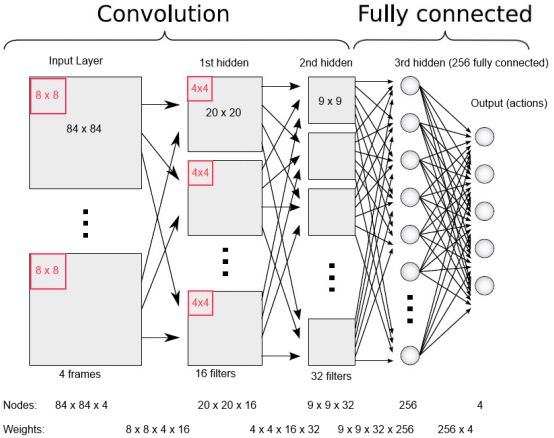
\includegraphics[scale=0.7]{img/structure}
			\centering
			\caption{DeepMind original topology \cite{repli}}
			\label{fig:topology13}
		\end{figure}
		
		In the 2013 paper from DeepMind \cite{ataridrl}, the network structure seen in figure \ref{fig:topology13} was used. This was later extended to the network structure seen in figure \ref{fig:topology15} in 2015 when published in Nature.\\
		
		\begin{figure}[h]				
			\includegraphics[scale=0.27]{img/structure2}
			\centering
			\caption{DeepMind extended topology}
			\label{fig:topology15}
		\end{figure}
		
		For this implementation, I have chosen the 2013 DeepMind topology, as it has been proven to work in this application to a broad set of video games, and is less complex than it's 2015 counterpart in terms of computation. This topology takes in four greyscale images of size 84x84, and then applies four filters of size 8x8, with stride of 4 \textbf{MAY NEED TO EXPLAIN STRIDE IN EARLIER SECTION}, to produce sixteen feature maps of size 20x20 in the second layer. These filters are applied as local receptive fields, which as explained in the earlier section on neural networks, sweep across the image with many pixels of the image, or neurons in the case of the network, sharing the weights of the filter(s).\textbf{This could be explained above instead if not already?!?} The second layer then is also a convolutional layer, and applies two filters of size 4x4, with stride 2, to produce thirty-two feature maps of size 9x9 in the third layer. This third layer is then connected to the fourth layer, which is a fully connected layer of size 256. \textbf{Explain FullConn Layer in NN theory?!?!} The fourth layer then connects to the final layer which is fully connected and is of varying size depending on the amount of actions available in the game the network is being applied to.\\
		
		It's worth noting that this convolutional neural network does not have any pooling layers. This is due to the nature of the images being used for this network application, Atari 2600 games screens are low resolution images. Max pooling layers would have been used had this network been applied to images that were of a higher resolution.
		
		\begin{figure}[h]				
			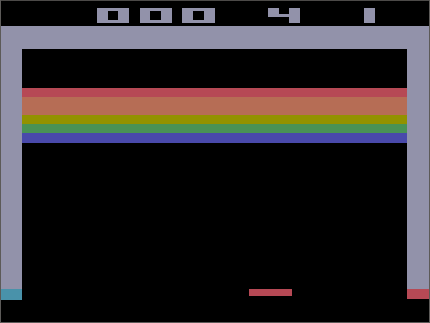
\includegraphics[scale=0.5]{img/screenshot}
			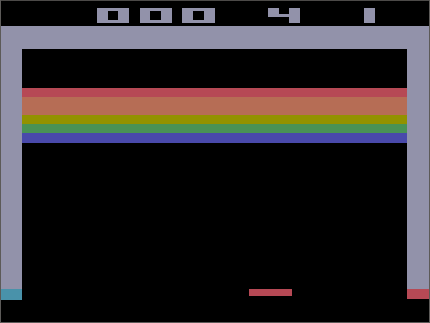
\includegraphics[scale=0.5]{img/screenshot}
			\centering
			\caption{Screenshot of the Atari 2600 game `Breakout' compared to a real-life image.\textbf{CHANGE TO REAL LIFE IMAGE (2ND ONE)}}
			\label{fig:screenshot}
		\end{figure}
	
	\medskip
	
	\subsection{Learning}
	%Replay memory, rmsprop/backprop, q learning.
		The network will learn overall using the reinforcement learning method of Q-learning, making it a deep q-network. The backpropagation learning for the network will use a technique known as RMSProp (Root mean square propagation) \cite{rms}.
		\begin{algorithm}
			\caption{Q-Learning element \cite{humanlevel}}
			\label{algo:qlearn}
			\begin{algorithmic}[1]
				\State Sample random minibatch of transitions ($\phi_j,a_j,r_j,\phi_{j+1}$) from $\mathcal{D}$
				\State Set $y_j =
					\begin{cases}
   						r_j& \text{for terminal } \phi_{j+1}\\
    					r_j + \gamma \text{max}_{a'}Q(\phi_{j+1},a';\theta),& \text{for non-terminal } \phi_{j+1}
					\end{cases}$
				\State Perform a gradient descent step on $(y_j - Q(\phi_j,a_j;\theta))^2$
			\end{algorithmic}
		\end{algorithm}
		
		From the main algorithm in algorithm \ref{algo:agentAlgo}, the learning is done in the section extracted in algorithm \ref{algo:qlearn}. Here, after stochastically selecting samples from the minibatch in line 1, we get an estimate on future rewards from line 2, and then perform a gradient descent step in line 3.\\
		
		The gradient descent step allows the network to know how much to alter the weights in the network when it performs backpropagation. The technique of RMSProp being used for the backpropagation is a variation of Stochastic gradient descent which will ``divide the learning rate for a weight by a running average of the magnitudes of recent gradients for that weight" \cite{rms}.
	
	\bigskip

\section{Implementation sprints}
	The development of this project was done in a series of sprints, as it was done using the agile software model (See section 5.1 - Software life-cycle).
	
	\subsection{Methods to manipulate I/O}
	%See Gregynog presentation and beyond
		The first sprint for the implementation was establishing a method to enable communication between C++ and the Arcade learning environment. This is accomplished by including and using a class known as the \textit{ALEInterface}, with consistent methods across both the C++ and Python such as those seen in the example code in Code Listing 1.\\
		
		The interface with ale needs to be initialised, from that we can then load in the game ROM (a .bin file specified either in the code itself or when run from the command line) and then get information about this game. We can get either the legal or minimal set of actions for the video game (both stored in a structure known as \textit{ActionVect}). The legal action set are all actions available to the player when playing the game whereas the minimal action set is the smallest subset of the legal actions needed to play the game. In the context of the neural network, the action set will be the size of the output layer. Once we have a decision on the action to be taken, we will perform the act command with the chosen action, which will return the reward obtained in the game from the given action. 	 
		
		\renewcommand{\lstlistingname}{Code Listing}
		\begin{lstlisting}[caption={ALEInterface in C++},label={ALEIO}]	
#include <ale_interface.hpp>

int main(int argc, char* argv[]) {

	//Initialise interface with environment
	ALEInterface ale;
	
	//Set whether game screen/sound will be displayed
	#ifdef __USE_SDL
		ale.setBool("display_screen", false);
		ale.setBool("sound", false);
	#endif

	//loads specified game 
	ale.loadROM(argv[1]); 

	//gets legal actions for game
	ActionVect legalAct = ale.getLegalActionSet();

	//performs action and returns reward
	int reward = ale.act(legalAct[0]);
	
	//returns whether game has ended or not
	bool gameOver = ale.gameOver();

	//returns game screen data
	ALEScreen screen = ale.getScreen();	
}

		\end{lstlisting}
			
		We can then also get a boolean value of whether the game has reached a game over state, as well as getting game screen information. This is output as a size 210x160 \textit{ALEScreen} structure of unsigned characters, which are 8-bit hexadecimal values representing a corresponding colour from a 128-colour palette specific to the Atari 2600.\\
		
		Initially small dummy C++ classes were made to test communication with the Arcade learning environment, with it being attached to the neural network at a later sprint.
	\medskip
	
	\subsection{Preprocessor}
	%Discuss how it later got implemented to newer version of ALE (prerelease version on Git).
	
	As the output from the Arcade learning environment does not exactly match the expected input to the neural network, some preprocessing steps are required. Much like with the communication with the arcade learning environment, this was at first done with some dummy C++ classes before being added the the larger network later on.\\
	
	The preprocessor crops the image and converts to greyscale (with use of a look-up table) using Algorithm \ref{algo:preprocess}.
	
		\begin{algorithm}[h]
			\caption{Region of Interest and greyscale conversion}
			\label{algo:preprocess}
			\begin{algorithmic}[1]
				\State ALEScreen screen = ale.getScreen();
				\State constant int ROI\textunderscore TOP = 32; constant int ROI\textunderscore BOT = 18;	
				\State int width = screen.width(); int height = screen.height();
				\State Image img;
				\State
				\State int jt = 0;
				\For{(int j = ROI\textunderscore TOP; j \textless height - ROI\textunderscore BOT; j++)}
					\For{(int i =0; j \textless width; j++)}
						\State int pix = screen.get(j, i);
						\State img[jt][i] = GREYSCALE[pix];		
					\EndFor
					\State jt++;
				\EndFor
			\end{algorithmic}
		\end{algorithm} 
	It then downscales the resulting image by a rate of 0.525 using Algorithm \ref{algo:downscale}.
		
		\begin{algorithm}[h]
			\caption{Image downscaling}
			\label{algo:downscale}
			\begin{algorithmic}[1]
				\State constant int DESIRED\textunderscore IMAGE\textunderscore XY = 84;
				\State constant int INPUT\textunderscore IMAGE\textunderscore XY = 120;
				\State double scaleRatio = INPUT\textunderscore IMAGE\textunderscore XY;(double)DESIRED\textunderscore IMAGE\textunderscore XY;
				\State int newX, newY;
				\State Image newImg;
				\State
				\For{(int y=0; y \textless DESIRED\textunderscore IMAGE\textunderscore XY; y++)}
					\For{(int x=0; x \textless DESIRED\textunderscore IMAGE\textunderscore XY; x++)}
						\State newY = floor(y*scaleRatio);
						\State newX = floor(x*scaleRatio);
						\State newImg[y][x] = img[newY][newX];				
					\EndFor
				\EndFor
			\end{algorithmic}
		\end{algorithm} 
		
	The resulting data is now ready to be input to the neural network.\\
	
	It is worth noting that the data type \textit{Image} is defined as $vector<vector<int>>$ in this project.
	\medskip
	
	\subsection{Network generation}
	%Algorithms, standardised functions, library?
	%initially hard coded, now extendable/standardised
	
	The neural network structure, based off the work of DeepMind and as seen in figure \ref{fig:topology13}, has 3 convolutional layers, followed by two fully connected layers.\\ 
	
	As a result, there exists two kinds of neurons, a standard Neuron to be used in fully connected layers, and a Convolutional Neuron to be used in convolutional layers. The convolutional neuron, defined as class \textit{ConvNeuron}, inherits from the standard \textit{Neuron} class for this Neural network project. Both kinds of neurons hold information on their value and their connections.\\
	
	The convolutional (input, first hidden, and second hidden) layers hold information on the filter(s) to be applied, that is the amount of filters, the size of the filter(s), the stride at which to apply them and the filter(s) themselves. A \textit{Filter} data type in the case of this project is defined as $vector<vector<double>>$ and are held in the data type \textit{Filters}, which is defined as $vector<Filter>$. The convolutional layers also hold the neurons for that layer, stored in a data type called \textit{FeatureMap} which is defined as $vector<vector<ConvNeuron^*>>$.\\
	
	The fully connected (third hidden, and output) layers hold a \textit{Weights} data structure which is defined as $vector<double>$, as well as a \textit{NeuronSet} defined as $vector<Neuron^*>$.\\
	
	The constructor for the neural network will feed in the input image(s), weights, and game actions size). The input image(s) are received from the game after being preprocessed, the game actions size is also received from the game. The weights are randomly initialised outside of the network before being fed in. The weights are held in a structure known as \textit{weightStruct} which holds two \textit{Filters} data types and 2 \textit{Weights} data types. The weights for the first pass of the neural network are initialised randomly, and will be tuned then as the network learns. The structure to hold to weights is outside of the network so that the agent can update then as it learns and then feed them into the network.\\
	
	As for the creation of the neural network itself, the methods to generate the network are generalised, allowing the network structure to be altered at any time easily, granted that the input layer is convolutional and the network consists of only convolutional and fully connected layers. The pseudo code for generation of a input convolutional layer can be seen in algorithm \ref{algo:inputLayer}.\\
		
		\begin{algorithm}[h]
			\caption{Input convolutional layer generation pseudocode}
			\label{algo:inputLayer}
			\begin{algorithmic}[1]
				\Procedure{ConvLayer(Images, filter size, number of filters, stride)}{}	
				\For{each image}
					\For{y-axis values of image}
						\For{x-axis values of image}
							\State Create new convolutional-Neuron
							\State Set value to pixel at [j][i] in image
							\State Store convolutional-neuron in feature map
						\EndFor
					\EndFor
					\State Add feature map to feature map collection in layer
				\EndFor
				\EndProcedure
			\end{algorithmic}
		\end{algorithm}
		
		The input convolutional layer differs from it's non-input counterparts in that it have no previous layer, it will take in the Images instead of the outputted feature maps of a previous layer, and does not need to take into consideration any weights, summation or activations to it's neurons. The pseudo-code for the generation of a non-input convolutional layer can be seen in algorith \ref{algo:noninputLayer}.\\
		
		\begin{algorithm}[h]
			\caption{Non-input convolutional layer generation pseudocode}
			\label{algo:noninputLayer}
			\begin{algorithmic}[1]
				\Procedure{ConvLayer(Previous layer, filter size, number of filters, stride)}{}	
				\State Store pointer to previous layer
				\For{each feature map}				
					\For{each filter to be applied}					
						\For{y-axis values within image where filter is applied}						
							\For{x-axis values within image where filter is applied}							
								\State Create new convolutional-neuron
								
								\For{y-axis of filter}								
									\For{x-axis of filter}
										\State Add connection to previous layer using weight from filter										
									\EndFor									
								\EndFor
								\State Store convolutional-neuron
							\EndFor							
						\EndFor
						\State Add feature map to feature map collection in layer
					\EndFor					
				\EndFor
				
				\EndProcedure
			\end{algorithmic}
		\end{algorithm}
		The amount of non-input convolutional layers can be easily specified then in the neural network, so the network is not stuck to one static structure.\\		
		
		The pseudocode for the creation of a fully connected layer that is connected to from a convolutional layer can been seen in algorithm \ref{algo:convtofcLayer}. \\

		\begin{algorithm}[h]
			\caption{Fully connected layer generation  pseudocode}
			\label{algo:convtofcLayer}
			\begin{algorithmic}[1]
				\Procedure{FullConnLayer(previous layer, layer size)}{}	
				\For{size of layer}
					Create new Neuron 
					\For{each neuron in previous layer}
						\State add connection between new neuron and previous convolutional neuron
					\EndFor
					\State Add Neuron to layer
				\EndFor
				\EndProcedure
			\end{algorithmic}
		\end{algorithm}
		
		These constructors are then called in the neural network to define the structure of the neural network and create it. In the case of my neural network, class variables are used in the network class to hold the layers, constants are defined for variables such as filter sizes and counts, and the generation of the layers is done in the layer class constructors. The code to generate the network topology outlined in the 2013 DeepMind paper would look like code listing \ref{netGen} if no constants were used.
				\renewcommand{\lstlistingname}{Code Listing}
		\begin{lstlisting}[caption={Network generation},label={netGen}]	
SetInputLayer(ConvLayer(m_input, 8, 4, 4));
m_inputLayer.SetFilters(m_firstWeights);

SetSecondLayer(ConvLayer(m_inputLayer, 4, 2, 2));
m_secondLayer.SetFilters(m_secondWeights);

SetThirdLayer(ConvLayer(m_secondLayer, 0, 0, 0));

SetFourthLayer(FullConnLayer(m_thirdLayer, 256));
m_fourthLayer.SetWeights(m_thirdWeights);

SetOutputLayer(FullConnLayer(m_fourthLayer, GetActionSetSize()));
m_outputLayer.SetWeights(m_fourthWeights);
}

		\end{lstlisting}

	\medskip
	
	\subsection{Network feedforward}
	Now that we can generate the network, the network needs to have data input and then propagate that data forward to make a decision. The forward propagation of the network is done by calling the \textit{activateNeurons()} function of each non-input layer in sequential order.\\
	
	 The \textit{activateNeurons()} function of a layer will loop through every neuron in the layer and call the neuron's \textit{CalculateValue()} function. This function loops through all of the connections in the neuron, at performs a summation on them to get the value for the neuron. After that, the \textit{Activation} function is called on the neuron which performs the non-linear rectifier activation on the Neuron.\\
	
	Once this has been performed all the way up to the output layer, the network will have it's decision values in each neuron of the output layer. To get the decision of the network in the agent, the agent calls the network's \textit{getDecision()} function which returns the index of the neuron which has the highest value.
	\medskip
	
	\subsection{Backpropagation}
		This crucial element of the neural network was sadly not completed and implemented, due to time constraints couple with several difficulties in understanding how to implement it for a network of this kind.\\		
		
		One such difficulty is the first step of error backpropagation, determining the error for each of the output neurons. The target value for the network, as determined by the intelligence agent, is the index of the neuron that the network should have given the highest value to. However, in error backpropagation, each individual output neuron needs to have a an individual error calculated. I am unsure how to do so when we are only trying to determine that one of the neurons should have a higher value than the others.\\
		
		Another difficulty was in implementing the propagation back through the network. The objective of backpropagation is to tune the weights of the network to be able to achieve a more accurate output decision of the network. However in the first implementation of the network, the connections just stored the values of the weights, so when propagating backwards the network was unable to tell where the weights came from to be able to update them. As well as this, in the case of convolutional layers, weights are shared across multiple neurons, so it is necessary to store either a pointer to the weights or an index value.\\
		
		When implementing a pointer to the weight, the network generated much slower, which would become detrimental when it came to applying this network to the game. An attempted solution using the index values of the weights was implemented, however due to time constraints it was unable to be verified working and then have the backpropagation implemented with it. One issue I foresaw using the index value in the connection for the weights was that the convolutional layers used 2-dimensional weight (and neuron) structures whereas the fully connected layers used 1-dimensional weight (and neuron) structures. This would mean I may have had to hard code the backpropagation process rather than having a preferred generalised version of the code so that the implementation could be easily extended with a network structure change.\\

		
		As a result of this element of the network being missing, the neural network being developed in C++ is not viable to be able to learn to play video games, as the fundamental \textit{learning} element of the network is missing, the network would only be able to make random actions with no ability to improve it's efforts.
	\medskip
	
	\subsection{Replay Memory}
		The replay memory for the intelligence agent allows us to keep a collection of previous transitions taken by the agent. These transitions consist of:
		\begin{itemize}
			\item Current state (screen) of the game.
			\item Action chosen by network.
			\item Reward received from game.
			\item Following state (screen) of the game.
			\item Whether the current state of the game is terminal.
		\end{itemize}
		
		This replay memory has two main functions, \textit{AddTransition()}, and \textit{GetMiniBatch()}.\\
		
		The \textit{AddTransition()} function takes in the transition as a parameter, and will store it within the replay memory data structure. The replay memory itself has a finite size, so if it is at capacity, it has will remove replace existing transitions, in a first-in-first-out fashion.\\
		
		The \textit{GetMinibatch()} function will return a $vector<transition>$ structure holding a stochastic sample of transitions known as a \textit{minibatch}, with the size of the minibatch specified as a constant.\\
		
		The replay memory of the network was implemented, however the learning process in the agent that would have utilised it was not.
	\medskip
	
	\subsection{Python library*}
	
	\medskip
	
	\subsection{Artificial Intelligence Agent*}
		%when plugging the network on, issue with images/weights input to network.
	\medskip	
	
	\subsection{Training the network*}
		\textit{Although this did not occur, existing implementations state that this process can take 3-5 days (make sure to get these as references). Explain why this was problematic late on in the project.}

	\bigskip
\section{Reflection of results*}

	\bigskip

\section{Suggestions for further work*}

\newpage
\printbibliography[
	    heading=bibintoc,
        title={References}
    ]
\newpage
\appendix

\section{Appendix: Facts and figures}
	Use the table from human level control paper, however also include any changes to values for the implementation, i.e. minibatch size. [hyperparameters]
	
	Also include the results graph from human level.

\section{Appendix: Class diagrams}


\end{document}

